\section{Shape Matching}
\label{sec:shapeMatching}

This section presents a set of matching functions to determine if two shapes originate from the same geometry within the RANSAC tolerance. Only shapes of the same type can be matching. Hence, it is not necessary to define functions to match for example a plane shape with a cone shape since the result will always be false. 
Shape matching is performed on two primitive shapes that are detected by Schnabel et al.'s algorithm. It is a key part of the clustering process in Section \ref{sec:shapeClustering}. 


\subsection{Elementary Matching Functions}
\label{sec:elementarMatchingFuns}

As the primitive shapes are represented by only a handful of parameters, it is sufficient to determine a similarity measure (called \textit{matching}) of these parameters. First, elementary matching functions for numbers, vectors, positions, and axes are defined. Since matching is an approximation of equality, each matching function's result is determined by comparing a computation result to a threshold $\lambda$. If a matching function returns \verb|true| (i.e., the values don't deviate more than the given threshold), the input values are considered to be matching. 

\begin{itemize}
    \item \textbf{Matching floats $f_1, f_2$}: 
        $$\frac{f_1}{f_2} \geq \lambda, \textrm{ where } f_1 \leq f_2$$  
    \item \textbf{Matching vectors $v_1, v_2$}: 
        $$\frac{v_1}{|v_1|} \cdot \frac{v_2}{|v_2|} \geq \lambda$$
    \item \textbf{Matching positions $p_1, p_2$}: 
        $$\sqrt{(p_1.x - p_2.x)^2 + (p_1.y - p2_y)^2 + (p_1.z - p_2.z)^2} \leq \lambda$$
    \item \textbf{Matching axes $a_1, a_2$}: 
    \\
    An axis is defined by a start and end point. Let $p_{01},p_{02}$ be the start and end point of $a_1$ and $p_{11}, p_{12}$ the start and end point of $a_2$. Furthermore, let $v_1, v_2$ be the direction vectors of $a_1$ and $a_2$. The rays of the axes are denoted as $r_1 = p_{00} + sv_1$ and $r_2 = p_{10} + tv_2$. The closest distances for start and end point for each axis to the complementary ray are calculated. From those four values, the largest value $d$ is used for decision making. The matching decision is composed as follows: 
        $$\frac{v_1}{|v_2|} \cdot \frac{v_2}{|v_2|} \geq \lambda_1 \land d \leq \lambda_2$$
\end{itemize}


\subsection{Primitive Shape Matching Functions}
\label{sec:primitiveShapeMatchingFuns}

With the elementary matching functions defined in Section \ref{sec:elementarMatchingFuns}, it is easy to define matching functions for two primitive shapes based on the elementary matching functions:

\begin{itemize}
\item \textbf{Matching plane shapes}: 
A plane shape consists of a quad that encloses all support points. For distance computation, the plane is used rather than the quad, as the quad is limited to the shape's points. For each corner of each quad, the distance to the other plane is calculated. From those eight values, the largest distance $d$ is chosen. Two plane shapes are matching if the planes' normal vectors are matching in regards to a threshold value $\lambda_1$ and $d$ is smaller than or equal to a threshold value $\lambda_2$.
\item \textbf{Matching cylinder shapes}: 
A cylinder consists of an axis and a radius. Two cylinder shapes are matching if radii and axes are matching. 
\item \textbf{Matching cone shapes}:
Cones consist of an axis, an apex, and an opening angle. Two cone shapes are matching if the axes, apexes and opening angles are matching. 
\item \textbf{Matching sphere shapes}: 
Two sphere shapes are matching if the center positions and the radii are matching. 
\item \textbf{Matching torus shapes}: 
A torus consists of a center position, an axis and a major and minor radius. Two torus shapes are matching if the center position, axes, major radii, and minor radii are matching. 
\end{itemize}

The matching result heavily depends on the chosen threshold values. Table \ref{tab:matchingThresholds} shows the $\lambda$ values that are used for this implementation. Plane matching uses a custom heuristic that is not depicted in the table. For this heuristic, $\lambda_2 = 0.05$ is chosen. Note that matching floats is a relative measure, whereas matching positions and axes compares absolute distances. Matching vectors uses the angle between the two vectors to calculate a matching. 

\begin{table}
\centering
\begin{tabular}{ r | r }
    Matching  & threshold values \\
  \hline
  Floats    & $\lambda = 0.99$ \\
  Vectors     & $\lambda = 0.95$ \\
  Positions    & $\lambda = 0.05$ \\ 
  Axis        & $\lambda_1 = 0.95$, $\lambda_2 = 0.05$\\  

\end{tabular}
\caption[Different threshold values for parameter matching]
{The different threshold values for parameter matching.}
\label{tab:matchingThresholds}
\end{table}


\section{Shape Clustering}
\label{sec:shapeClustering}


Shape detection is performed on individual octree nodes from different levels of detail. Thus, the size of the detected shapes is limited to the extent of the octree node. While on a low level of detail, a wall may be contained by a single octree node, on a higher level, a node will only contain parts of the wall, and multiple nodes contain primitive shapes that originate from the same wall. 

\par

Given a base shape selected by the user, the clustering algorithm aims to find matching primitive shapes and build a larger coherent cluster of primitive shapes over multiple levels of detail. Oesau et al. \cite{oesau2016planar} propose a graph-based clustering for shapes to detect coplanar shapes. Our shape-clustering algorithm works similarly, but is not limited to planes. The octree is searched for primitive shapes that were detected previously and that match the base shape. From this set of shapes, a complete graph is created, and a region-growing algorithm reduces the number of shapes to those that create a coherent shape cluster. 


\subsection{Building a set of matching primitive shapes}
\label{sec:matchingSetBuilding}

The cluster is constructed from primitive shapes that are currently visible. Therefore, rather than searching in the original octree, the octree culled at the render horizon is queried. Matching shapes are found by traversing the octree and returning those shapes that match the base shape. The base shape, selected by the user, has a particular level of detail. For the shape cluster to mimic a structure of a similar level of detail, only shapes from nodes are used whose level of detail does not deviate more than a user-specific threshold $l$. Let $l_0$ be the level of detail of the base shape, only shapes are considered whose level of detail lie in the range of $[l_0 - l ; l_0 + l]$. Hence, a threshold $l = 0$ only allows for shapes of the same level, $l = 2$ allows for shape from two levels above and below the base shape's level of detail to be considered. Using a threshold value of 0 creates small clusters, as larger overlapping shapes cannot form bridges between smaller shapes. While testing, the threshold $l = 2$ creates large enough clusters include meaningful parts of a structure, while still having little to no unwanted shapes in the cluster. Shapes with the largest extent from the lowest level of detail hardly get clustered as they usually differ significantly from the smaller shapes. 

\par

This set of shapes already creates a cluster where each primitive shape can be seen as a part of a larger shape. However, the distances between the shapes are not yet taken into account. Thus, gaps between the shapes may still exist. Figure \ref{fig:cuboids} shows the case of two cuboids, whose front face share a plane. By only using the matching functions to create a cluster, both front faces are packed into the cluster, even though there is a visible gap between them.
For sphere and torus shapes, this step is sufficient to create a coherent cluster, since both shapes are finite. For infinite shapes, an additional step is performed using a graph-based region growing algorithm.

\begin{figure}
    \centering
    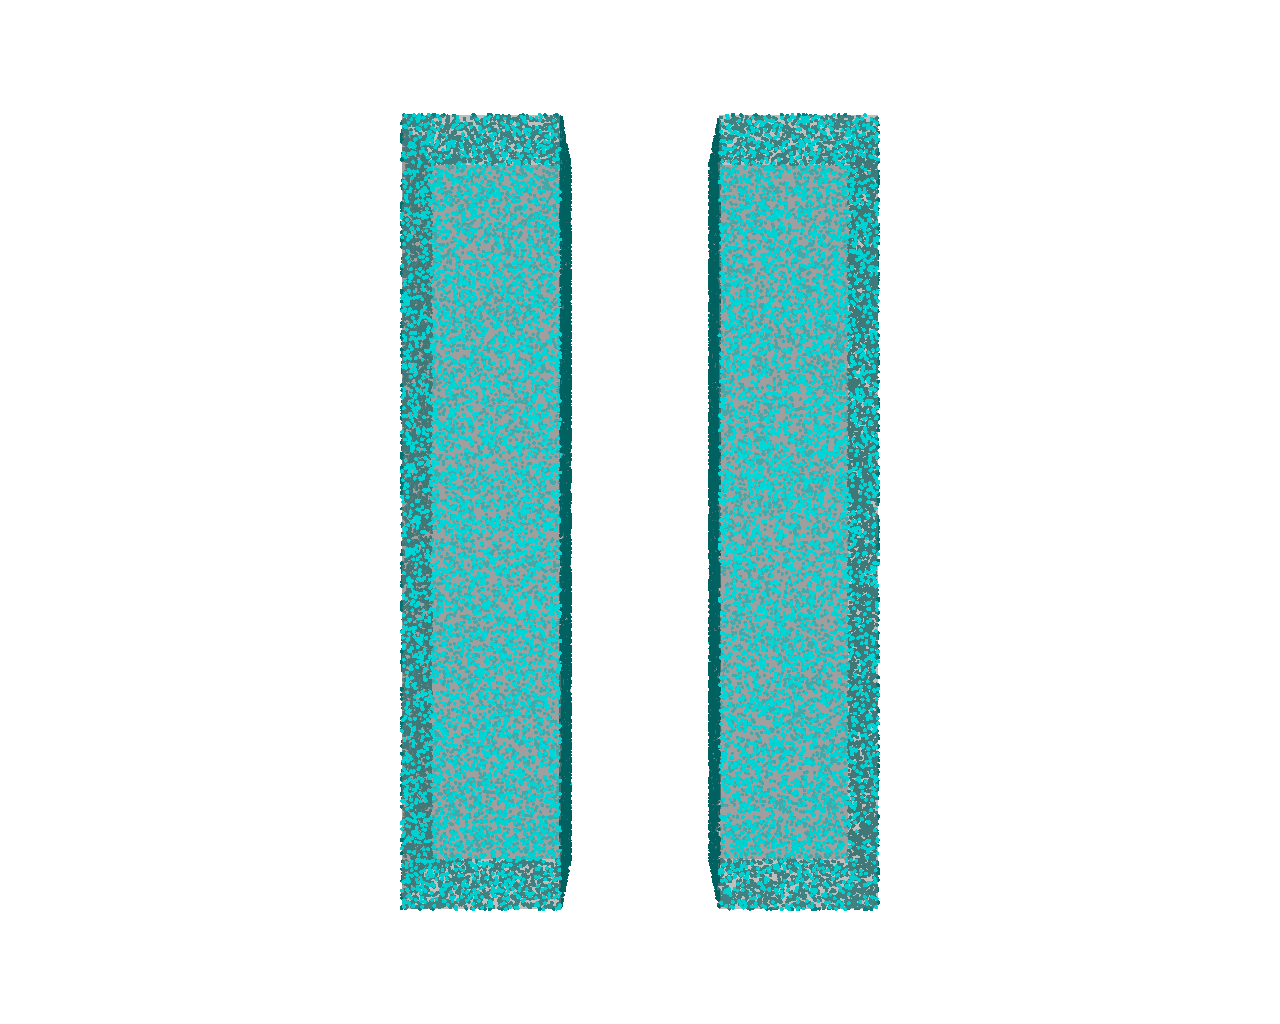
\includegraphics[width=0.6\textwidth]{Shape_Detection/cuboids.png}
    \caption[Point cloud consisting of two cuboids.]
        {A generic point cloud of two cuboids. The detected planes are rendered in grey.}
    \label{fig:cuboids}
\end{figure}


\subsection{Graph-based Region Growing}
\label{sec:regionGrowing}

A cluster of shapes can be seen as an $\epsilon$-connected component from a larger graph. A complete graph is created using all matching shapes, as well as the base shape, as vertices. In a complete graph, an edge exists between any pair of vertices. The weight of an edge is determined by a distance function for each primitive shape:

\begin{itemize}
    \item \textbf{Plane Shape}: As a plane shape is bounded by a quad, the distance between two plane shapes is computed as the shortest distance between the two bounding quads.
    \item \textbf{Cylinder Shape}: The shortest distance between two cylinder shapes is determined by the shortest distance between all pairs of start/end points of both cylinders. 
  \item \textbf{Cone Shape}: The shortest distance between two cone shapes is determined by the shortest distance between all pairs of start/end points from both cones. 
\end{itemize}

Overlapping shapes can occur when shapes from multiple levels of detail are clustered. However, this causes no problems for the clustering process, as the distance between two overlapping shapes is set to $0$.
A cluster is created by growing a region in a graph, adding only vertices that connect to the current region via an edge whose weight is smaller than $\epsilon$. This creates a cluster of shapes, ensuring that the distance to the closest neighboring shape is at maximum $\epsilon$. 

\begin{figure}[h]
    \centering
    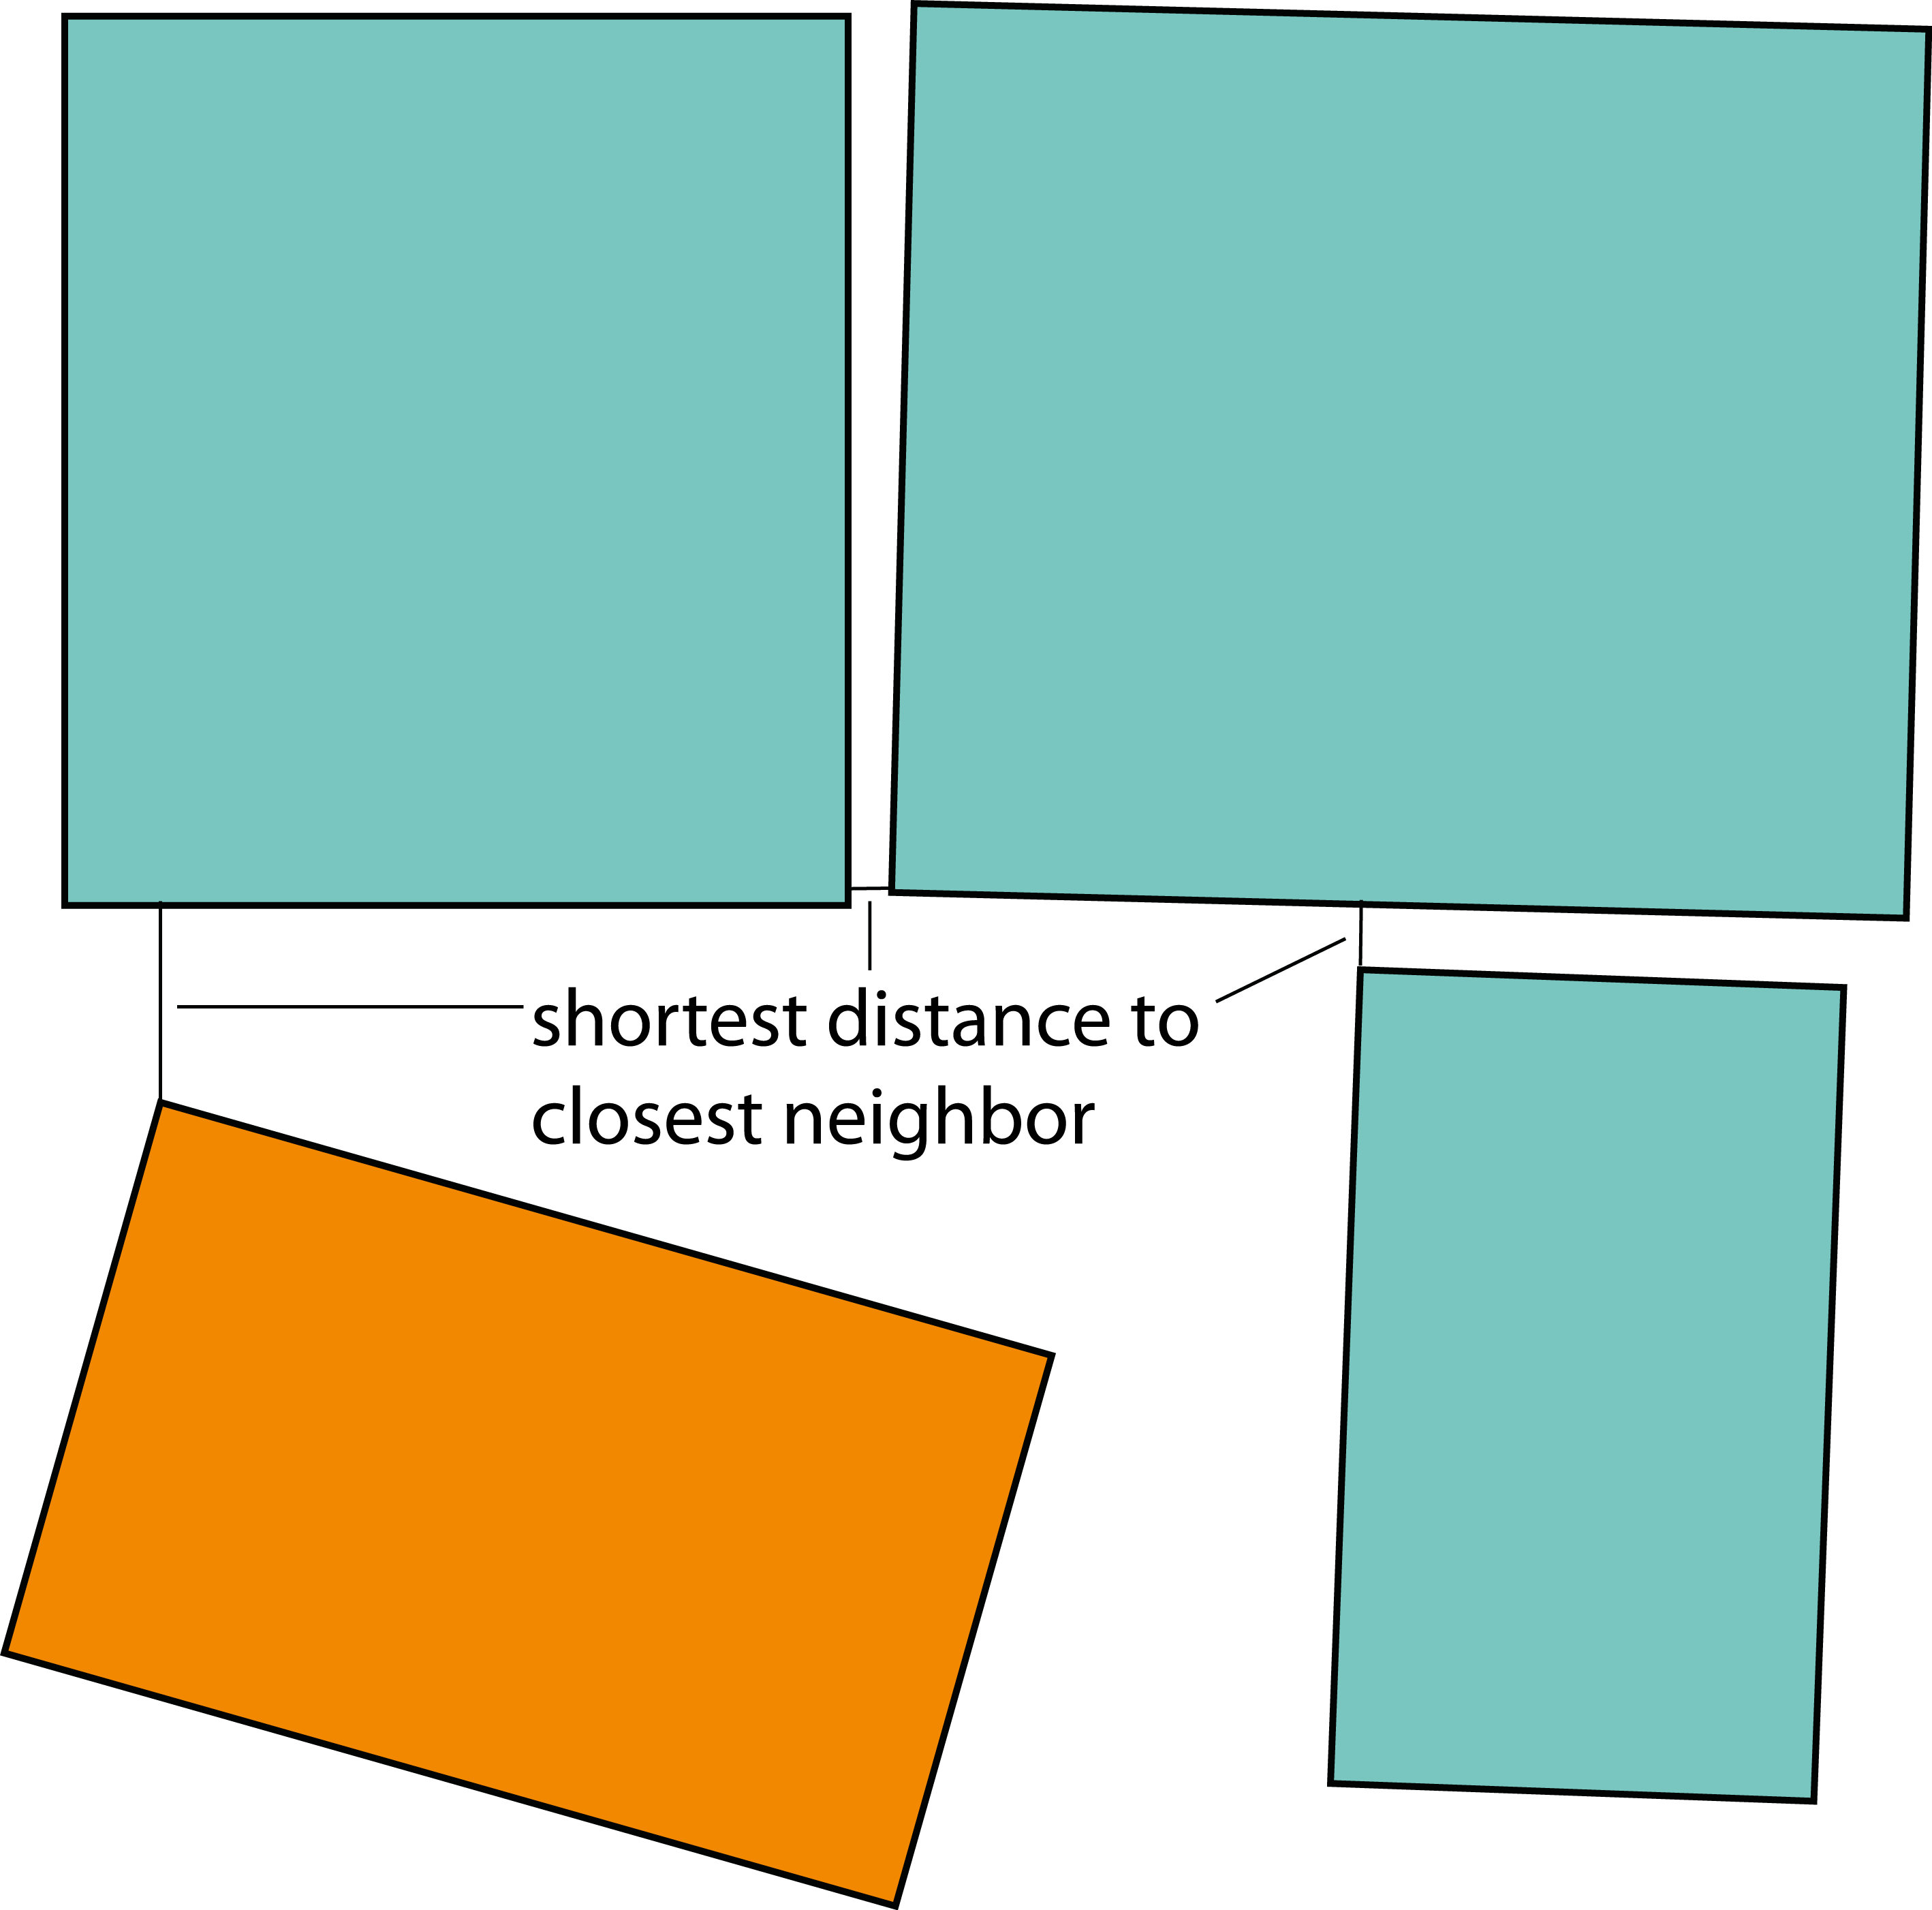
\includegraphics[width=0.6\textwidth]{Shape_Detection/regionGrowingPlanes.png}
    \caption[Exemplary $\epsilon$-connected plane cluster]
        {A cluster of plane shapes created by computing the $\epsilon$-connected component. The base shape is colored in blue. Planes that belong to the cluster are colored in turquoise. Shapes that do not belong to the cluster are colored in orange. The cluster's $\epsilon$ distance is drawn in grey. Each shape that intersects this area belongs to the cluster.}
    \label{fig:regionGrowingPlanes}
\end{figure}

\begin{figure}
\centering
\subcaptionbox{ \label{fig:regionGrowingCylinder}}{%
  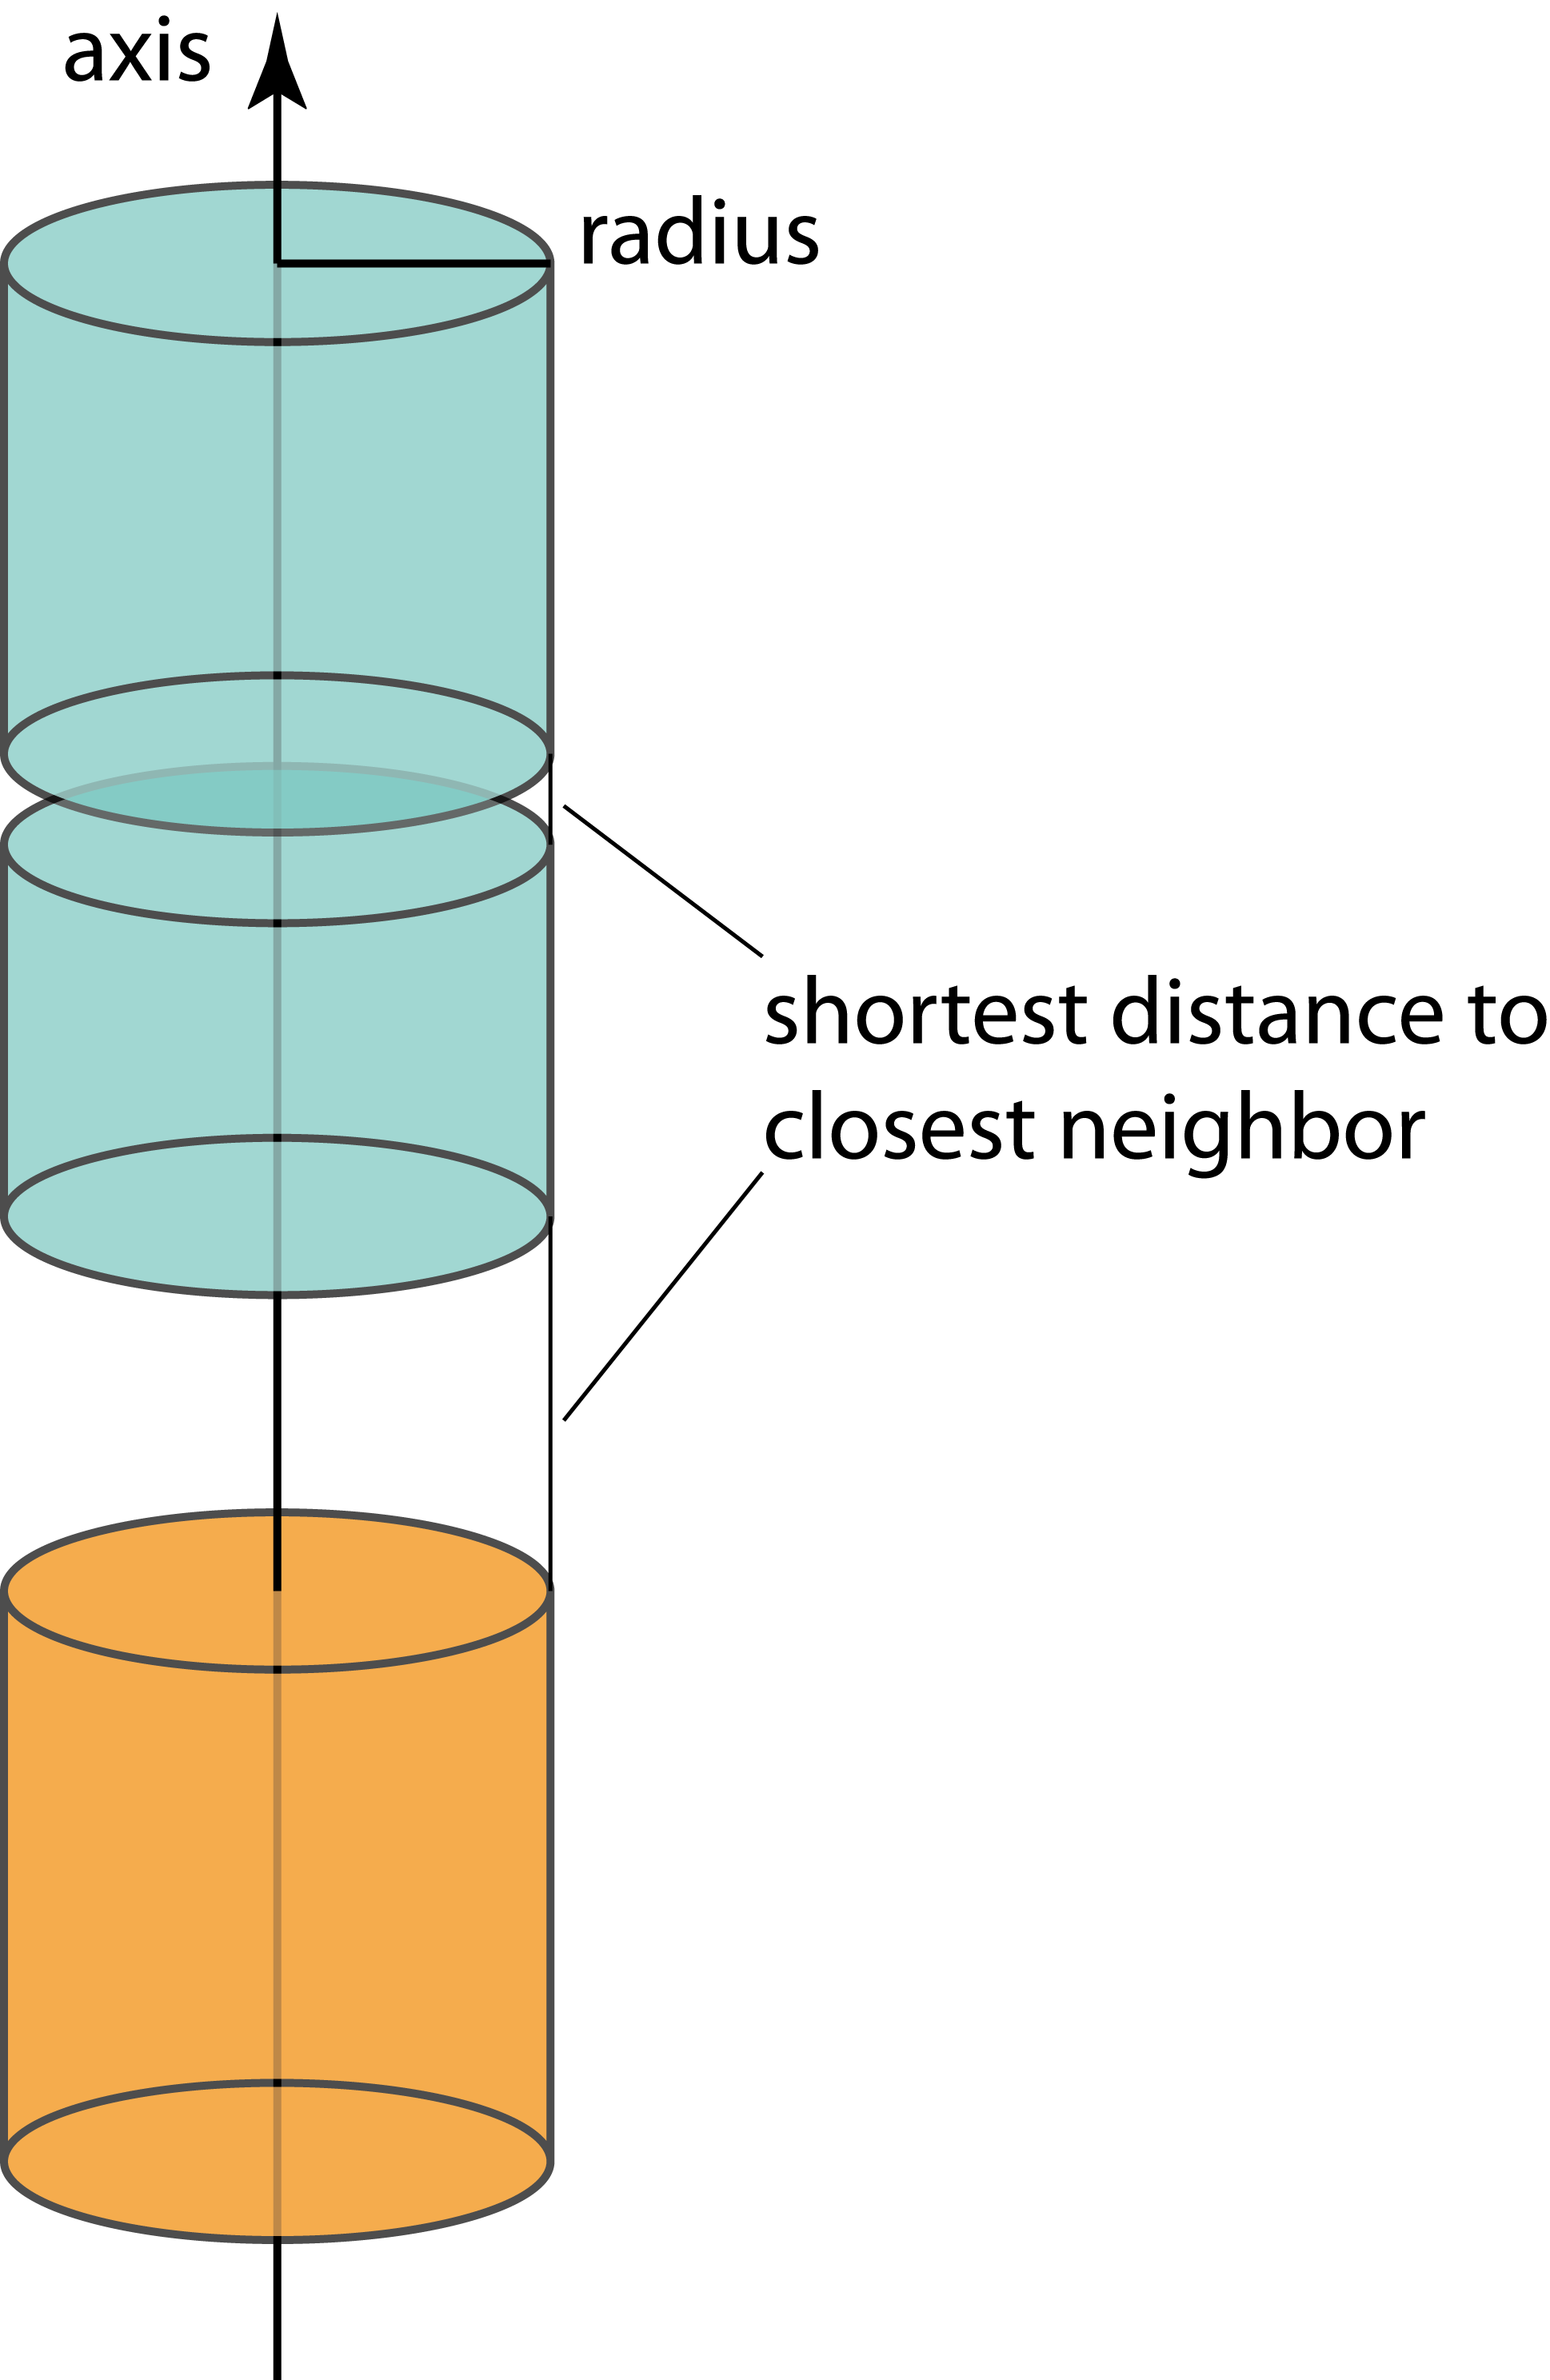
\includegraphics[width=0.3\textwidth]{Shape_Detection/regionGrowingCylinder.png}%7
  }
\subcaptionbox{ \label{fig:regionGrowingCone}}{%
  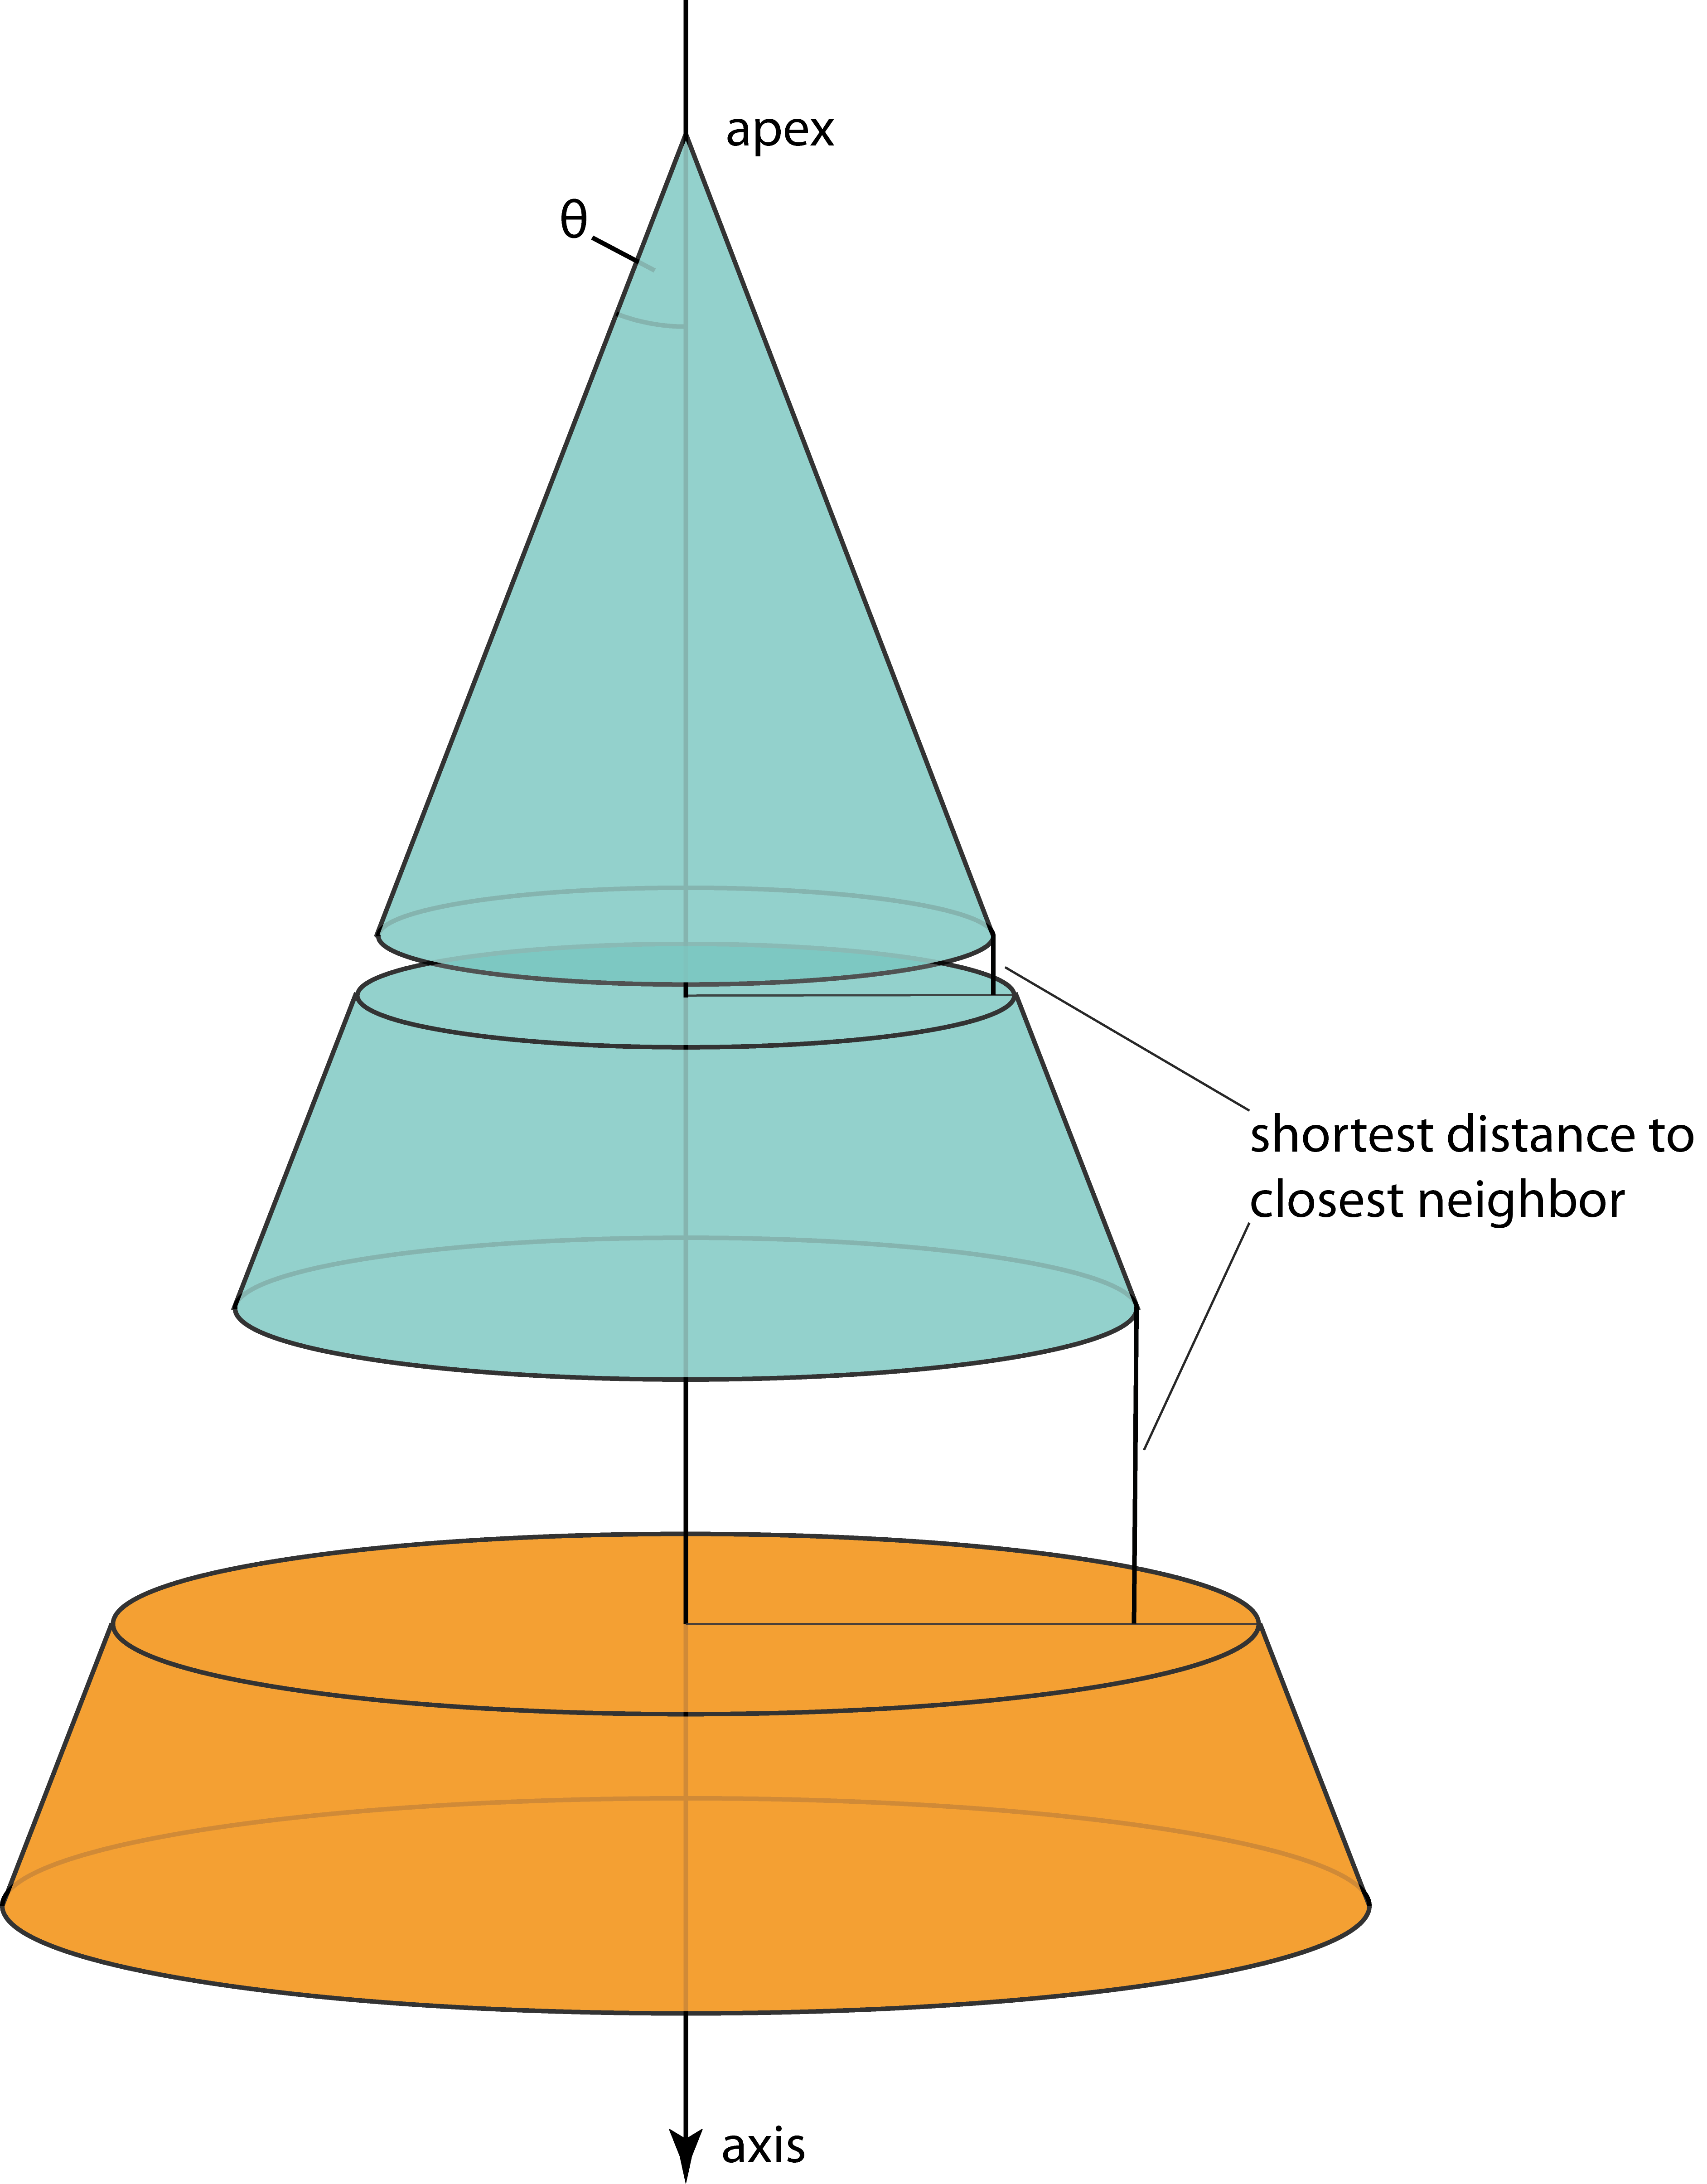
\includegraphics[width=0.5\textwidth]{Shape_Detection/regionGrowingCone.png}%
  }
    \caption[Exemplary cylinder and clone cluster]
        {This figure shows a cylinder cluster and a cone cluster build from matching shapes. Shapes that belong to the cluster are colored in turquoise.}
    \label{fig:regionGrowingConeCylinder}
\end{figure}

Figure \ref{fig:regionGrowingPlanes} shows an exemplary illustration of region growing for plane shapes. The distance between two plane shapes is measured as the closest distance between the two bounding quads.

\par

Figure \ref{fig:regionGrowingConeCylinder} showcases region growing for both cylinder shapes and cone shapes. The matching heuristic already confirms that the shapes lie on the same axis and share a similar radius. Therefore, instead of a three-dimensional world distance, a one-dimensional distance between two points is sufficient to build a shape cluster. 

\par

The region-growing component of the clustering heavily depends on the $\epsilon$ distance threshold. A proper distance threshold that mirrors the region's topology well is the density of an octree node as described in Section \ref{sec:shapeDetectionParameterSelection}. For this task, we chose the density of the node of the base shape, more specific: $\epsilon = 2 \cdot density $.